\section{Gaussian Process Model}\label{sec:gpmodel}

GP can be applied as probabilistic models to regression problems. Here we will use the GP model to generalise a grid of stellar models to a continuous and probabilistic function that maps inputs (i.e., initial mass, chemical composition, etc.) to observable quantities (i.e., effective temperature, surface gravity, radius, etc.).  We aim to use the GP model as a non-parametric emulator, that is emulating the comparatively slow calls to models of stellar evolution. 
%
We adopt the a tool package named \textsc{GPyTorch}, which is a GP framework developed by \citet{gardner2018gpytorch}. \textsc{GPyTorch} is a Gaussian process library based on an open source machine learning framework PyTorch (\url{https://pytorch.org}). This tool package provides significant GPU acceleration, state-of-the-art implementations of the latest algorithmic advances for scalability and flexibility, and easy integration with deep learning frameworks. Source codes and detailed introductions could be found on \url{https://gpytorch.ai}.

\subsection{Gaussian Process Application}

We start with a grid of stellar models containing $N$ models with a label we want to learn, for example model effective temperature, which we will denote with the general symbol $\bf y$, and a set of input labels $\bf X$ (e.g., mass, age, and metallicity).  We can use a GP to make predictions of the effective temperature (or $y$) for additional input values given by $\bf X_{\star}$.  The vector $\bf y$ is arranged ${\bf y} = \left(y_{i}, ... ,y_{N} \right)^{T}$ where the subscript label references the stellar model.  The input labels are arranged into a $N \times D$ matrix where $D$ is the number of input dimensions (e.g., $D=3$ for mass, age, and metallicity) so that ${\bf X} = ({\bf x}_{1}, ..., {\bf x}_{N})^{T}$ where ${\bf x_{i}} = (x_{1, i}, ..., x_{D, i})^{T}$.  The matrix of additional inputs $\bf X_{\star}$ has the same form as $\bf X$ but size $N_{\star} \times D$.

\citet{williams1996gaussian}, from which our description below is based, define a GP as a collection of random variables, where any finite number of which have a joint Gaussian distribution.  In general terms, GP's ({\bf Guy, please check " 's "}) may be written as
\begin{equation}
y({\bf x}) \sim \mathcal{GP}\left( m({\bf x}), {\bf \Sigma}\right),
\end{equation}
where $m({\bf x})$ is some mean function, and ${\bf \Sigma}$ is some covariance matrix.  The mean function controls the deterministic part of the regression and the covariance controls the stochastic part.  The mean function defined here could be any deterministic function and we will label the additional parameters, or hyperparameters, $\phi$.  Each element of the covariance matrix is defined by the covariance function or {\it kernel function} $k$ which has hyperparameters $\theta$ and is given by,
\begin{equation}
{\bf \Sigma}_{n, m} = k({\bf x}_{n}, {\bf x}_{m}),
\end{equation}
where the inputs ${\bf x}_{i}$ are $D$-dimensional vectors and the output is a scalar covariance.

As a GP is a collection of random variables, where any finite number of which have a joint Gaussian distribution, the joint probability of our data $\bf y$ is
\begin{equation}
p({\bf y} | {\bf X, \phi, \theta}) = \mathcal{N}(m({\bf X}), {\bf \Sigma}).
\end{equation}
If we want to obtain predictive distributions for the output $\bf y_{\star}$ given the inputs $\bf X_{\star}$ the joint probability distribution of $\bf y$ and $\bf y_{\star}$ is Gaussian and given by
\begin{equation}
p \left( \begin{bmatrix} {\bf y} \\ {\bf y_{\star}} \end{bmatrix} \right) = \mathcal{N} \left( \begin{bmatrix} {\bf X} \\ {\bf X_{\star}} \end{bmatrix} , \begin{bmatrix} {\bf \Sigma} & {\bf K_{\star} }\\ {\bf K_{\star}}^{T} & {\bf K_{\star \star}} \end{bmatrix}  \right), 
\end{equation}
where the covariance matrices $\bf \Sigma$ and $\bf K$ are computed using the kernel function so that
\begin{equation}
{\bf \Sigma}_{n, m} = k({\bf X}_{n}, \, {\bf X}_{m}),
\end{equation}
which is an $N \times N$ matrix.
\begin{equation}
{\bf K}_{\star \, n, m} = k({\bf X}_{n}, \, { \bf X}_{\star \, m}),
\end{equation}
which is an $N \times N_{\star}$ matrix, and finally
\begin{equation}
{\bf K}_{\star \star \, n, m} = k({\bf X}_{\star \, n},  {\bf X}_{\star \,m}),
\end{equation}
which is an $N_{\star} \times N_{\star}$ matrix.
The predictions of $\bf y_{\star}$ are again a Gaussian distribution so that,
\begin{equation}
{\bf y}_{\star} \sim \mathcal{N}(\bf \hat{y}_{\star}, \, \bf C),
\label{eq:pred}
\end{equation}
where 
\begin{equation}
{\bf \hat{y}}_{\star} = m({\bf X}_{\star}) + {\bf K}_{\star}^{T} \, {\bf \Sigma}^{-1} \, ({\bf y} - m(\bf X)),
\end{equation}
and 
\begin{equation}
{\bf C} = {\bf K}_{\star \star} - {\bf K}_{\star}^{T} \, {\bf \Sigma}^{-1} \, {\bf K_{\star}}.
\end{equation}

At point we can make predictions on model properties given a grid of stellar models using equation \ref{eq:pred}.  But these predictions will be poor unless we select sensible values for the form and hyperparameters of the mean function and covariance function.  In the following section we detail a number of kernel functions that will be tested against the data.  We will then discuss the method for determining the values of the hyperparameters to be used.

\subsection{GP Model Inputs and Outputs}

We aim to derive stellar parameters based on fundamental inputs of the model grid. As mentioned in Section~\ref{sec:grid}, our model grid has four independent fundamental inputs, i.e., mass, initial metallicity, initial helium fraction, and mixing-length parameter. Moreover, we need another input to describe the evolution and hence the GP model contents five input demissions. 

Regarding the evolution index, stellar age is not ideal because its dynamical range varies track by track. The fractional age is a choice. However, we find global parameters (e.g. effective temperature) sharply change as a function of fractional age around the 'hook' and the turn-off point as shown in the left panel of Figure~\ref{fig:eep}. This is because stars evolve in a relatively short time scale at these stages. We hence use an Equivalent Evolutionary Phase ($EEP$) following \citet{2016ApJS..222....8D} as the five fundamental input. Note that we define $EEP$ in a  different way from \citet{2016ApJS..222....8D}. 
%
On each evolutionary track, we compute the displacement between model $n$ and model $n-1$ on the $T_{\rm eff} - \log g$ diagram as
\begin{equation}\label{eq:disp}
\delta d_{n} = ((T_{\rm eff, n} - T_{\rm eff, n-1}) ^{2} + (\log g _{n} - \log g_{n-1})^{2}))^{f},
\end{equation}
and the total displacement of model $n$ from the ZAMS (model 0) can be calculated with
\begin{equation}
d_{n} = \sum_{i = 0}^{i = n} \delta d_{i} .
\end{equation}
On the same evolutionary track, $d_{n}$ is normalised to the 0 --1 range and defined as defined as $EEP$. For our stellar model grid, $EEP$ equals to 0 at the ZAMS and 1 on the RGB where $\log$ = 3.6 $dex$. The factor $f$ in Eq. \ref{eq:disp} is adjustable for modulating $EEP$ to avoid obviours gap in the data space, and we find that $f$ = 0.18 gives the best data distribution.
%
In Figure~\ref{fig:eep}, we demonstrate how the effective temperature changes with fractional age and $EEP$. It can be seen that the usage of $EEP$ significantly smoothes the sharp features at the 'hook' and the turn-off point.
We summary GP model inputs and outputs as below.
\begin{itemize}
\item GP model inputs and their dynamic ranges:
\item[] Mass ($M$ = 0.8 -- 1.2$\rm M_{\odot}$)
\item[] Equivalent Evolutionary Phase ($EEP$ = 0 -- 1)
\item[] Initial metallicity ([Fe/H]$_{\rm init}$ =  -0.5 -- 0.5 dex)
\item[] Initial helium fraction ($Y_{\rm init}$ = 0.24 -- 0.32)
\item[] Mixing-length parameter ($\alpha_{\rm MLT}$ = 1.7 -- 2.5)
\item GPR model outputs: 
\item[] Effective temperature ($T_{\rm eff}$) 
\item[] Surface gravity ($\log g$)
\item[] Radius ($R$)
%\item[] The large spacing ($\Delta\nu$)  
\item[] Surface metallicity ([Fe/H]$_{\rm surf}$)
\item[] Stellar age ($\tau$)
\end{itemize}
Thus, the GP model can be described as 
\begin{equation}\label{gprmodel}
{\rm Outputs} = f(M, EEP, ({\rm Fe/H})_{\rm init}, Y_{\rm init}, \alpha_{\rm MLT}). 
\end{equation}

\begin{figure*}
        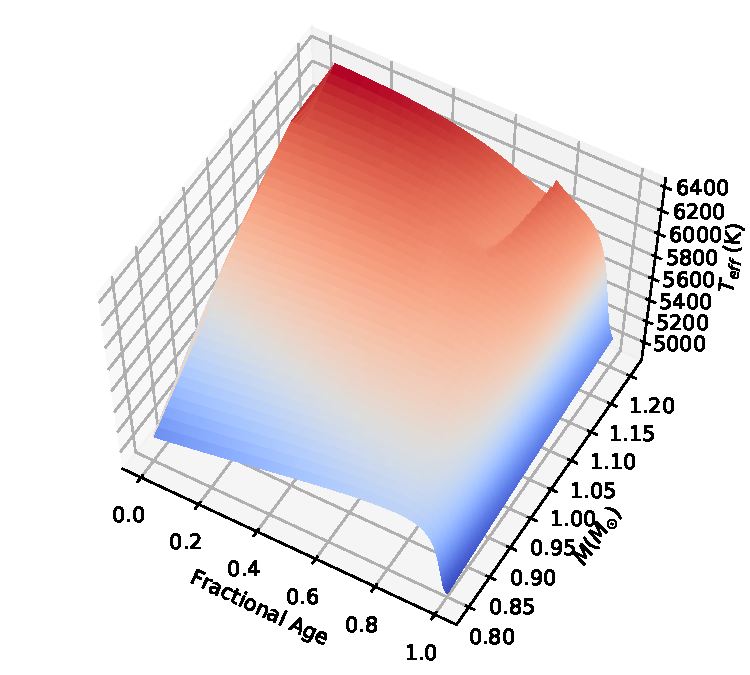
\includegraphics[width=1.\columnwidth]{2d_fage_data.pdf}
	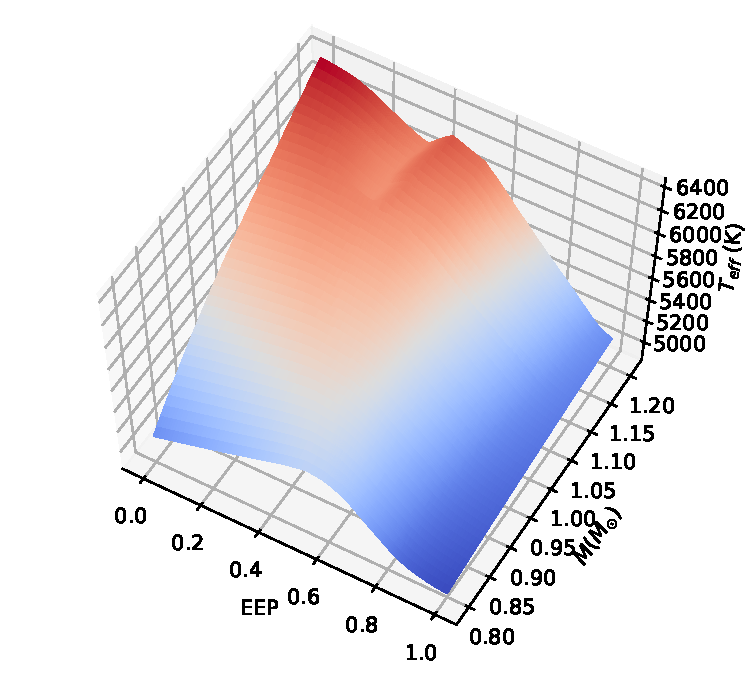
\includegraphics[width=1.\columnwidth]{2d_EEP_data.pdf}
     \caption{Surface plots of model effective temperature on the mass-fractional age (left) and mass-EEP (right) diagrams. Models in this figure are from the primary grid with fixed initial metallicity ($\rm [Fe/H]_{init}$ = 0.0), helium fraction ($Y_{\rm init}$ = 0.28) and mixing-length parameter ($\alpha_{\rm MLT}$ = 2.1). It can be seen that the effective temperature changes much smoother on the mass-EEP diagram at the hook and turn-off points.}
    \label{fig:eep}
\end{figure*}

\subsection{GP training Procedure}\label{workflow}
  
\subsubsection{Data Selection}

For training GP models properly, we need three types of data for training, validating, and testing GP models. 
%
Models in the primary and additional grids (as described in Table \ref{tab:grid}) are the training data. The off-grid models are divided 50-to-50 as validating and testing datasets . Note that validating and testing datasets are not on the same evolutionary tracks so they are independent to each other. 
%
%Validating dataset is for validating the GP model in the training process and is mainly used for early stopping, which is a form of regularisation for avoiding overfitting. We choose off-grid models but not on-grid models as validating data because the grid is equally spaced. Without additional information between grid points, an optimiser could either use a smooth function or a periodic function to fit the data and find no obvious differences in the likelihood. We describe how we use validating data in Section \ref{sec:training}. Lastly, testing dataset is independent on the training process and used for evaluating the final GP models. 

GP has limitation of the data size, because the computational and memory complexity exponentially increase with the number of data points.  In practice, typical data size for GP is on an order of $10^{4}$. Given that the grid contents $\sim 10,000,000$ models, only a small subset can be used. The sampling method is hence critical.
%
The evolve step is not the same at different evolutionary stages due to the \textsc{MESA} step-control strategy. For instance, stellar models are dense at the main-sequence and the red-giant phases but quite sparse on the subgiant stage. For this reason, a flat sampling is not appropriate.   
We test a few methods and find that using the displacement ($\delta d_{n}$) defined in Eq.~\ref{eq:disp} as the weight of sampling give a relatively uniform data distribution in the parameter space. 
%meets the above two requirements. 
%Firstly, we want the data to uniformly cover the parameter space for the best efficiency. Secondly, we need to highly weight models at phases where sharp changes present, e.g., models around the hook and turn-off points.   

\subsubsection{Training, Validating, and Testing GP Models}\label{sec:training}

The procedure contents two stages: training and testing.  
Training is the process that optimises hyperparameters with training dataset and validates the trained GP model with validating dataset. When training is completed, we test the GP model with testing dataset to quantify its accuracy.  
%
In the training process, we train and validate the GP model in every iteration. The model will be saved if it has the best validation result so far. The training process terminates when the validating result does not improve in the last 300 iterations. After training, we test the best GP model with the testing dataset. Details of the set up of training will be described in the following Section. 

Here we discuss the method for validating and testing a GP model. We do not use any popular methods, such like Root Mean Square Error (RMSE). Because we find that GP model performances are at similar accuracy level across the whole parameter space due to the differences in evolutionary features. We illustrate this with an example in Figure \ref{fig:2dtest}. As it can be seen that, we train a GP model which maps $M$ and $EEP$ to the effective temperature. The kernel function in the area of $M \geq 1.05 {\rm M_{\odot}}$ and $EEP \leq 0.7$ is more complex than that for other regions because of the appearance of the 'hook'. This particular area are relatively difficult to learn and hence poorly predicted by the GP model.
%
For other outputs, surface gravity and radius are similar to the case of effective temperature. The surface metallicity is not significantly affected by the hook, but it has a quick raise at the early subgiant phase in high-mass tracks. This is because high-mass tracks maintain shallow convective envelope and hence have strong diffusion effect during the main-sequence stage. Their surface metallicities at then end of the main-sequence are generally much lower than the initial value. When evolving to the early subgiant phase, the quick expansion of the surface convective envelope brings back the settling heavy elements to the surface. This results in a sharp raise of the surface metallicity after the turn-off point and GP models show relatively poor accuracy at this phase. 
%

When there is a subregion where a GP model perform worse than other areas, the error distribution is not Gaussian-like and hence a global estimator like RMSE is not suitable. What we need here is a simple method that reflects the general accuracy as well as the worst case.
We examine the error distribution as shown at the bottom of Figure \ref{fig:2dtest}. Errors of most data follows a Gaussian distribution but about $10\%$ data form long tails on both sides. For this case, the 68\% confidential interval is able to describe the accuracy of most data, and the 95\% and 99.7\% confidential intervals describe the median value and the length of the tail. Thus, we use the sum of three cumulative values at 68\%, 95\%, and 99.7\% of absolute errors as an error index to qualify GP models. For the case in Figure \ref{fig:2dtest}, cumulative values at 68\%, 95\%, and 99.7\% are 1.1, 4.9, and 11.1K, which give an error index equals to 17.1K. 

\begin{figure}
	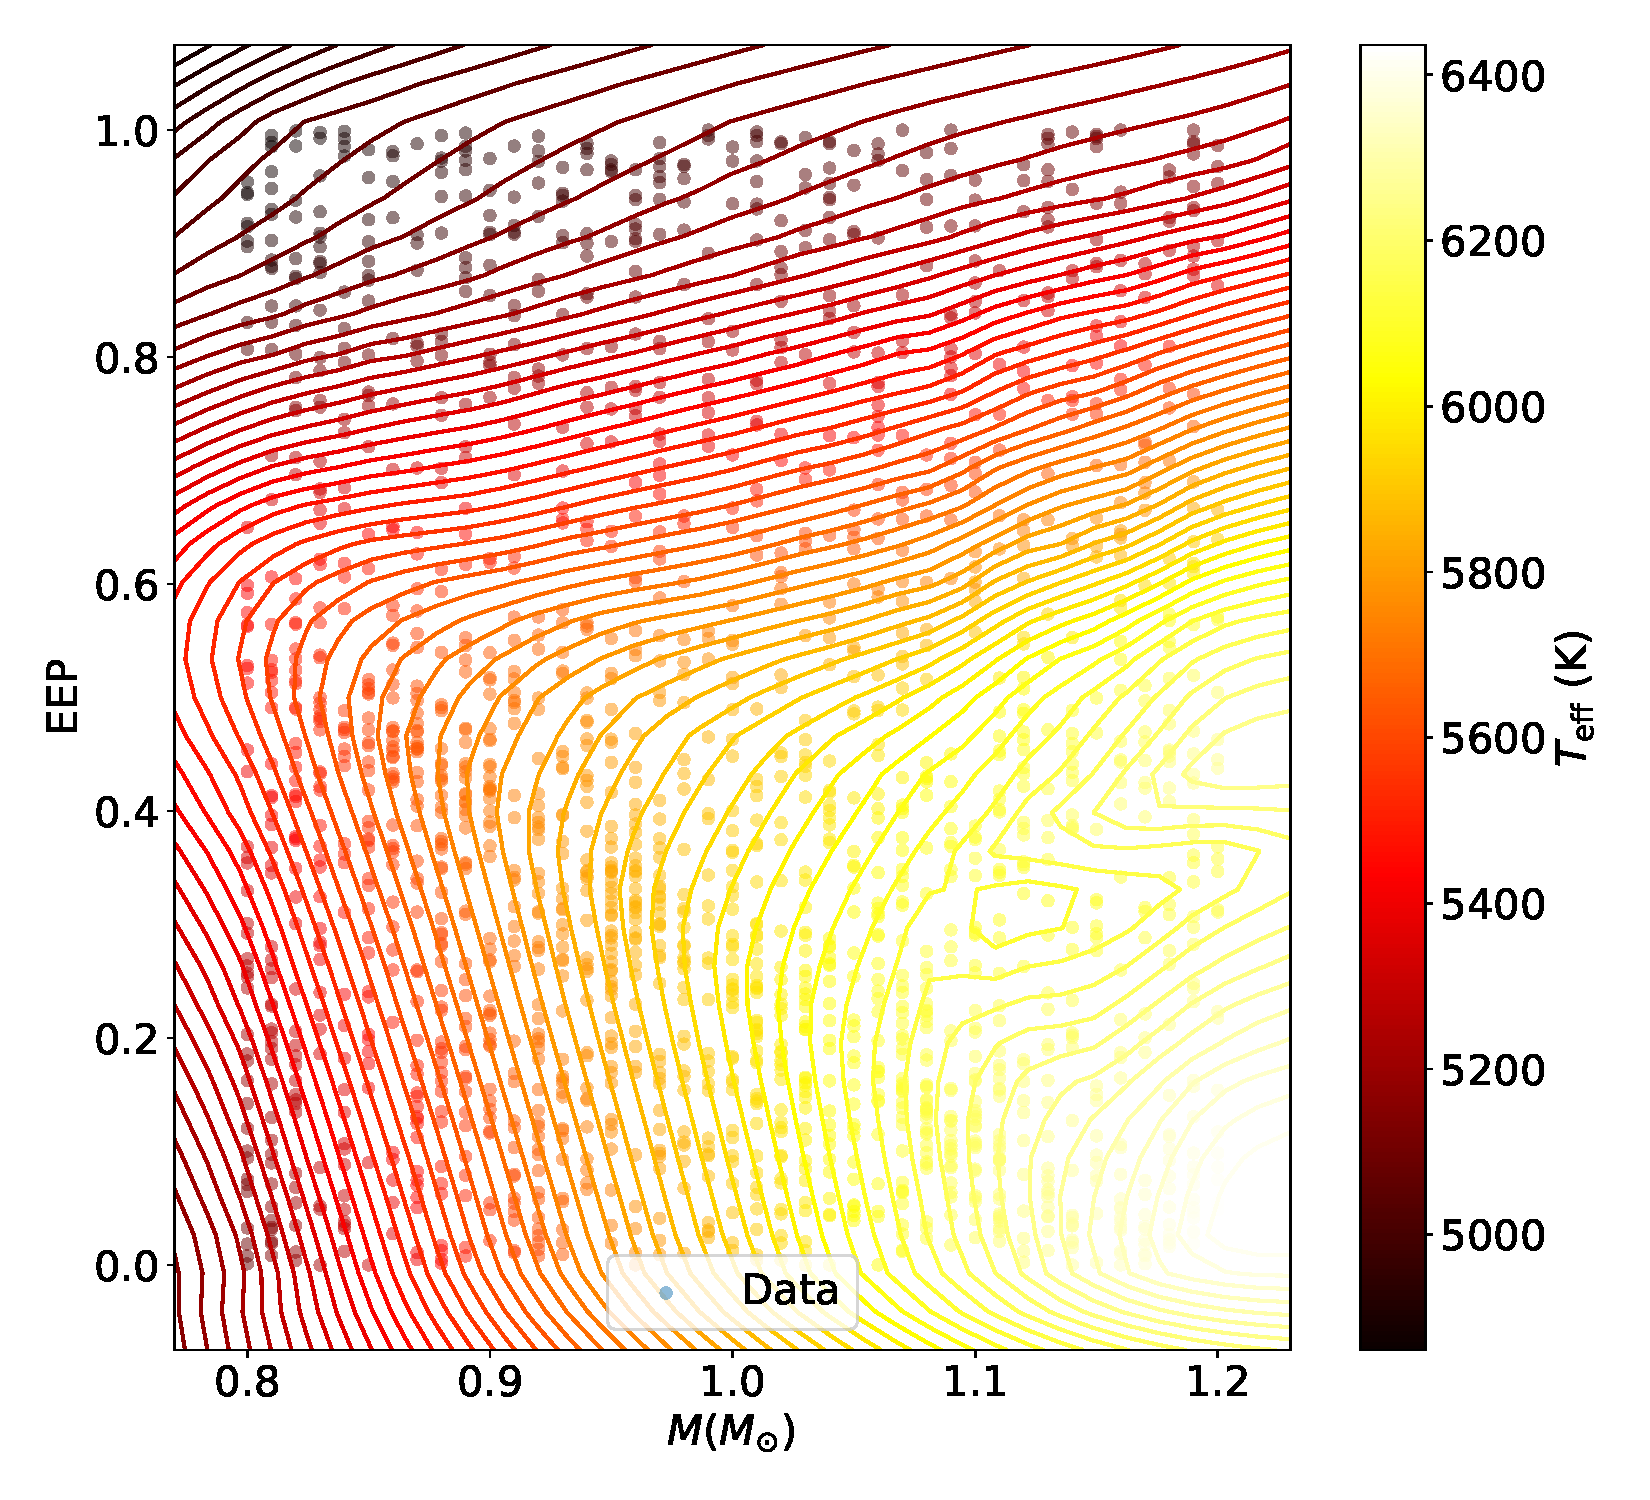
\includegraphics[width=1.0\columnwidth]{2d_GPmodel_function.pdf}
	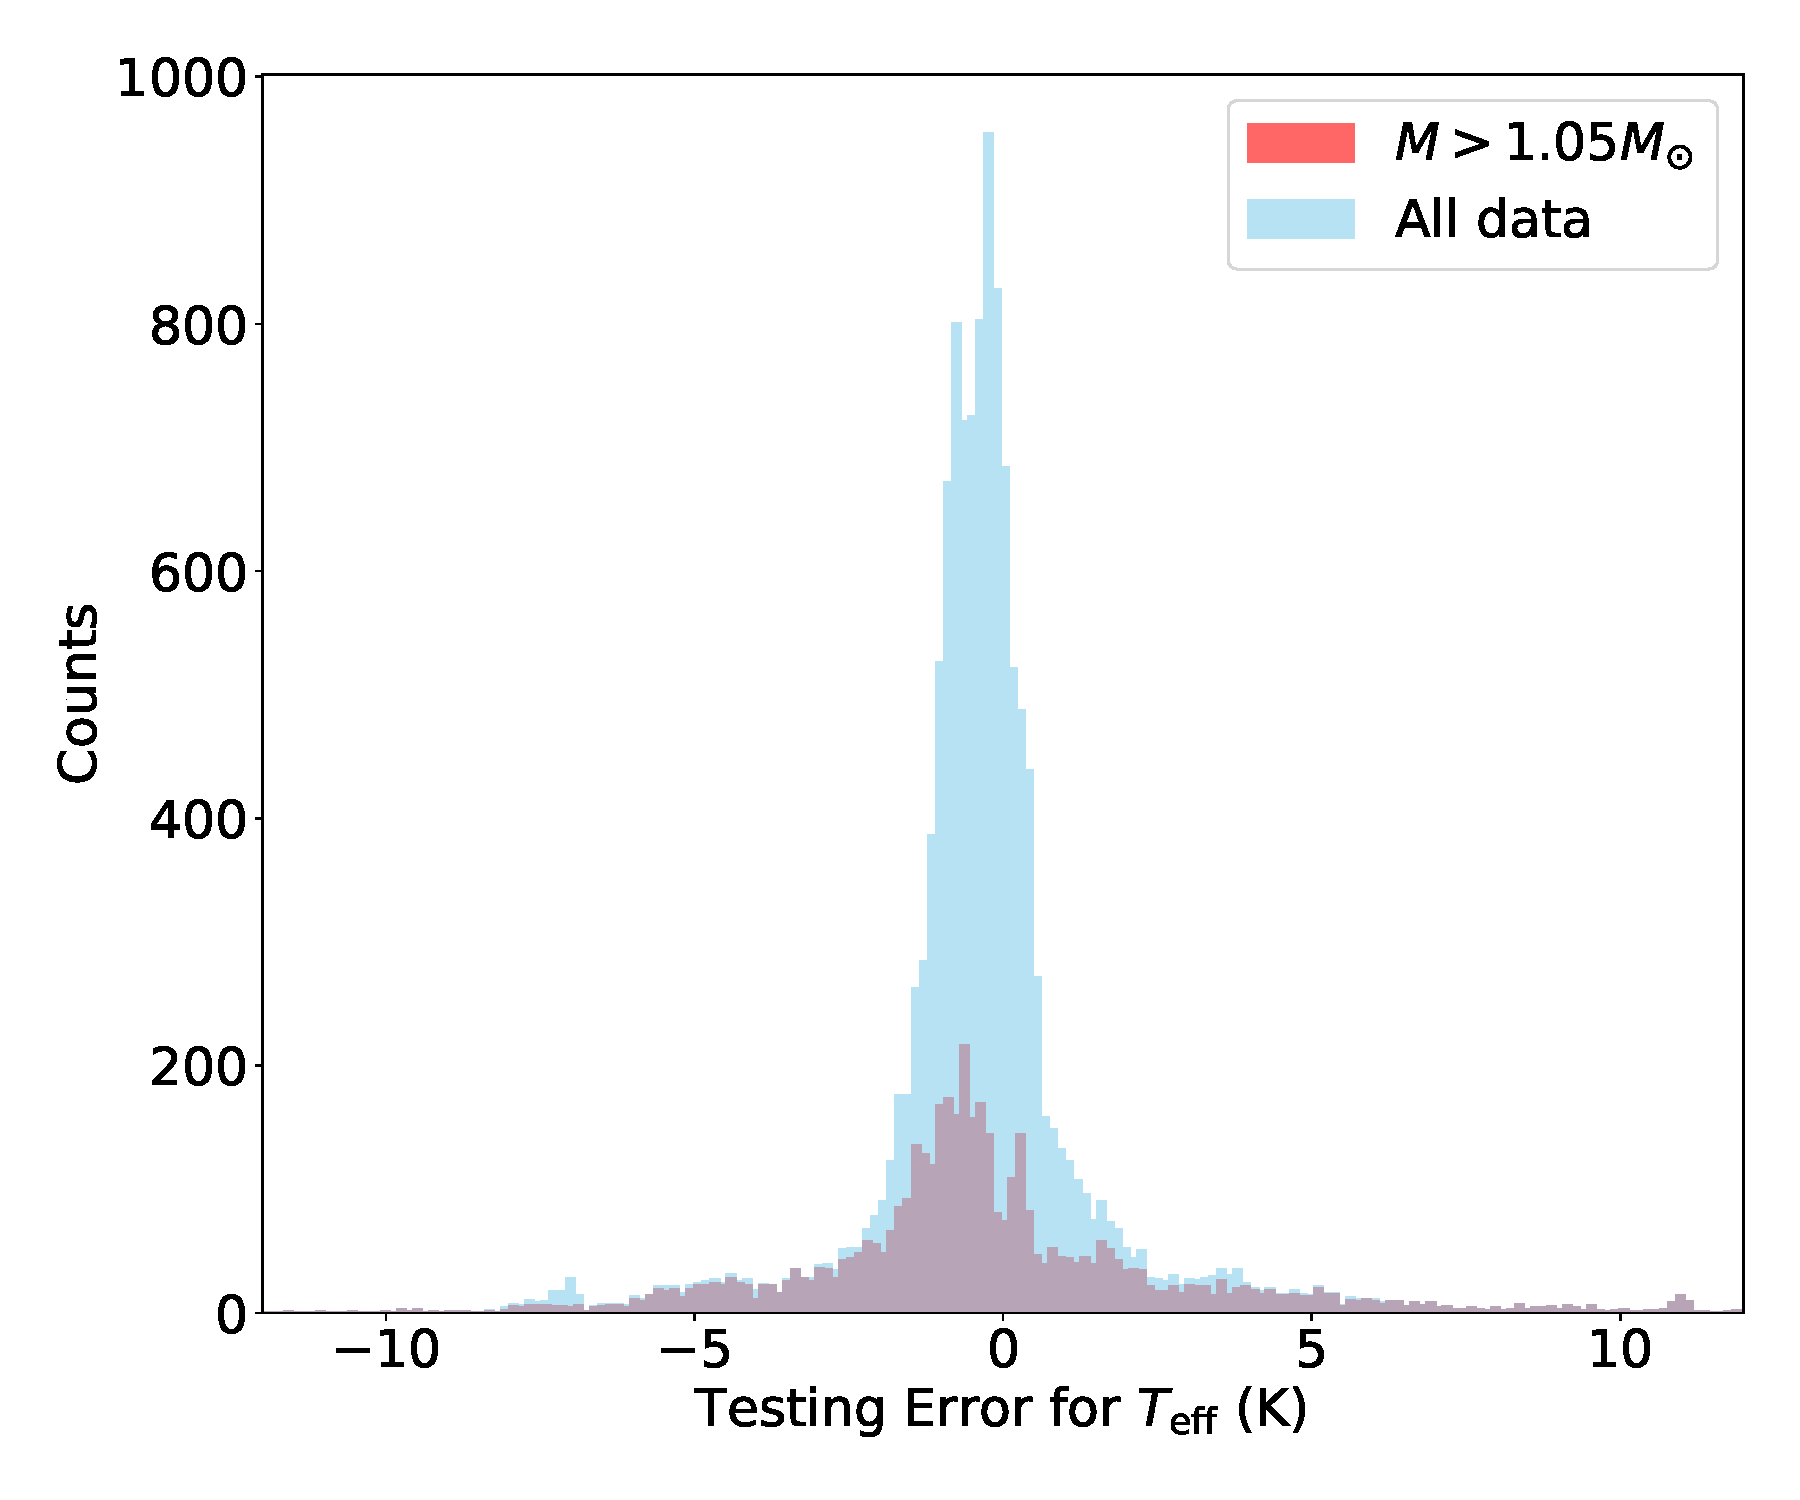
\includegraphics[width=1.0\columnwidth]{2d_testing_hist_effective_T.pdf}	
    \caption{Top: The 2D GP model for $T_{\rm eff}$. Bottom: probability distributions of validating errors of the GP model. }  
    \label{fig:2dtest}
\end{figure}


\subsection{Preliminary Tests and Settings of Training}

For training GP models, we need set up mean function, kernel, likelihood function, loss function, and optimiser. 
We do numbers of primary tests for comparing different options for the above elements and decide which to use. 
%
The primary tests are done on 2-demission (2D) GP models that content two inputs $M$ and $EEP$. The 2D GP models can be described as Outputs = $f(M, EEP)$. 
%
Training data for 2D GP models are selected from the primary grid with fixed [Fe/H]$_{\rm init}$ (0.0), $Y_{\rm init}$ (0.28), and $\alpha_{\rm MLT}$ (2.1). The training dataset contents 41 evolutionary track and 24,257 data points. We also computed 44 evolutionary tracks with same input [Fe/H]$_{\rm init}$, $Y_{\rm init}$, and $\alpha_{\rm MLT}$ but random $M$ for validating and testing. We use the sampling method mentioned in previous section and selected 20,000 data points for training, 10,000 for validating, and 10,000 for testing. 
%
The Exact GP approach is adopted and we test and develop our training training script based on the \textsc{Simple GP Regression} example in the \textsc{GpyTorch} package (\url{https://docs.gpytorch.ai/en/stable/examples/01_Exact_GPs/Simple_GP_Regression.html}).

\subsubsection{Mean Function}

We start with the mean function. As discussed above, evolutions of model outputs are not always smooth and can be complex in some areas. Although a GP model does not significantly affected by the choice of the mean function due to the flexibility of kernels, we find that a constant or linear mean function leads to a long time for training and a significant increase of the complexity of kernels. For this reason, we apply a Neural Network mean function which is flexible enough to map smooth as well as curved evolving features. We adopt an architecture includes 6 hidden layers and 128 nodes per layer. All layers apply the linear transformation to the incoming data. We apply the element-wise function (Elu) because it give relatively smooth mean functions. ({\bf may need ref for NN})

\subsubsection{Likelihood and Loss Function}

We then work on the likelihood function and the loss function. Our training object is a theoretical model grid. There is hence no observed uncertainty for each data point, but a tiny random uncertainty exists due to the approximations in the \textsc{MESA} numerical method. The noise model can be assumed as a Gaussian function with a very small deviation. 
%   
A likelihood specifies the mapping from latent function values $f(X)$ to observed labels $y$.
We adopt the the standard likelihood for regression which assumes a standard homoskedastic noise model whose conditional distribution is
\begin{equation}\label{eq:likelihood}
p(y|f(x)) = f + \epsilon, \epsilon \sim \mathcal{N}(0, \sigma^{2}),
\end{equation}
where $\sigma$ is a noise parameter. 
%
Given the random uncertainty is small, we use a small and fixed noise parameter and run a few tests. However, we find that it makes the GP models hard to converge and sometimes lead to obvious overfitting. When this noise parameter is set as free, it reduces to a small number anyway in the training progress because it is data-driven. For these reasons, we decide not put strict constraint for or prioritise this noise parameter and let the data determine. In practice, we only set up a loose upper limit ($\sigma$  < 0.1) for the noise parameter to speed up the training. One thing should be note that a GP model with a large noise parameter can not be a proper description for the stellar grid even if it gives good validating or testing errors. Because of this, we only adopt GP models with a noise parameter $\lesssim 10^{-4}$.   
The the loss function is simply the exact marginal likelihood in the logarithmic scale.

\subsubsection{Optimiser}

Afterwards, we run tests to decide the optimiser. We mainly compare two optimisers named SGD and Adam. Here SGD refers to Stochastic Gradient Descent, and Adam is a combination of the advantages of two other extensions of stochastic gradient descent, specifically, Adaptive Gradient Algorithm and Root Mean Square Propagation. 
%
The SGD optimiser in the \textsc{PyTroch} package involves the formula given by \citet{sutskever2013importance}. The formula makes it possible to train using stochastic gradient descent with momentum thanks to a well-designed random initialisation and a particular type of slowly increasing schedule for the momentum parameter. The application of momentum in SGD could improve its efficiency and make it less likely to stuck in local minimums. On the other hand, the Adam optimiser includes the \textsc{AMSGrad} variant developed by \citet{47409} to improve its weakness in the convergence to an optimal solution. With these new developments, the two optimisers give very similar results. We finally choose Adam because it works relatively efficiently and stable.  
%
We adaptive learning rate instead of a fixed value. Our training starts with a learning rate of 0.01 and decreases by a factor of 2 when the loss value does not reduces in the previous 100 iterations.    

\subsubsection{Early stopping}

We set up an early stopping for tow purpose: avoiding overfitting and terminating the training progress. 
The early stopping is controlled by validating results. When an optimal solution is found, the validating errors stop decreasing and then increase when overfitting happens. In the training process, we track the validation error index (introduced in Section~\ref{sec:training}) trigger the early stopping when the validation error index does not decrease in the previous 300 iterations. 

\subsubsection{GP kernels}

With the above set up, we lastly test for the best kernel for this work. We involved four basic kernels in the tests as listed below:
\begin{itemize}
\item RBF: Radial Basis Function kernel (also known as squared exponential kernel)
\item RQ: Rational Quadratic Kernel (equivalent to adding together many RBF kernels with different lengthscales)
\item Mat12: Matern 1/2 kernel (equivalent to the Exponential Kernel)
\item Mat32: Matern 3/2 kernel 
\end{itemize}
We applied each basic kernel and a couple combined kernels (RBF + Mat21, RQ + Mat21, Mat32 + Mat21, RBF + Mat32, RQ + Mat32) to train the 2D GP models. Among these kernels, the combined one RBF+Mat21 give the best fit to the training data, however, it does not give the best predictions for the validating and testing data. On the other hand, the GP model with the Mat32 kernel fit the training data reasonably well and its predictions have the best agreement with validating and the testing data. 
%
Comparing between the two kernels, the RBF+Mat12 Kernel is a combination of a smooth and a spiky kernel, which offers enough flexibility fit all features in the training data. However, the spiky function do not work well for off-grid regions. 
%
The smoothness of Mat32 kernel is somewhere between a spiky (Mat21) and a smooth kernel (RBF). It does not exactly fit some sharp features of the data but performs a good balance between on- and off-grid data. We hence adopted Mat32 kernels in our GP model.  

 \subsection{Strategy for Large sample}

The model grid we aim to train contents about 10,000,000 data points, which is much more than the upper limit of data size of the Exact GP (20,000). We hence consider other GP approaches. Our tests for the large-sample strategy are carried out with a 3-demission (3D) GP model, which have three fundamental inputs: $M$ and $EEP$ and  [Fe/H]$_{\rm init}$. The 3D model can be described as  (Outputs $ = f(M, EEP, {\rm [Fe/H]_{init}})$). 
Data for training 3D models (3D data hereafter) are from the primary grid with fixed $Y_{\rm init}$ (0.28), and $\alpha_{\rm MLT}$ (2.1). The training sample include 562 tracks and $\sim$ 300,000 data points. For validating and testing purposes, we compute another 174 evolutionary tracks with the same input $Y_{\rm init}$, and $\alpha_{\rm MLT}$ but random $M$ and [Fe/H]$_{\rm init}$. We firstly train an Exact GP model which includes 20,000 training data as the reference. 


We then consider the Stochastic Variational GP (SVGP) with \textsc{GPyTorch ApproximateGP} module. We train our data based on the SVGP example on \url{https://docs.gpytorch.ai/en/v1.1.1/examples/04_Variational_and_Approximate_GPs/SVGP_Regression_CUDA.html}. 
SVGP is an approximate scheme rely on the use of a series of inducing points which can be selected in the parameter space. It trains using minibatches on the training dataset and build up kernels on the inducing numbers. Underline principles and detailed descriptions of this approach can be found in \citet{hensman2015scalable}. The advantage of SVGP is the large capacity of sample size, however, the kernel complexities is still limited by the amount of inducing numbers. Moreover, because more training data is loaded and take off the memory, the SVGP model can only use 10,000 inducing points. This is to say, although more training data is used, the kernel complexity of the SVGP model is even simpler than the Exact GP model. As a result, the SVGP model does not improve the accuracy level.  For instance, the testing errors of $T_{\rm eff}$ at 68\%, 95\%, and 99.7\% are 2.0, 5.8, and 15.7 K (error index = 23.5 K) for Exact GP model and 2.2, 6.8, and 15.1 (error index = 24.1 K) for the SVGP model. Here we learn that SVGP is suitable for the case of large data sample but simple kernel complexity. 

We investigate another approach designed for the large dataset named Structured Kernel Interpolation (SKI GP). SKI GP was introduced by \citet{wilson2015kernel}. It produces kernel approximations for fast computations through kernel interpolation and is a great way to scale a GP up to very large datasets (100,000+ data points). We follow the example on \url{https://docs.gpytorch.ai/en/stable/examples/02_Scalable_Exact_GPs/KISSGP_Regression.html} to develop our script. We run a few tests to train a 3D SKI GP model with 100, 000 training data. Compare with the Exact GP and SVGP, its testing errors of $T_{\rm eff}$ are slightly improved to 2.0, 6.1, and 14.8 $K$ (error index = 22.9 $K$). However, the further test on the 5-demission data is not ideal: a SKI GP model with 100,000 training data performs much worse than an Exact GP model with 20,000 training data. The poor behaviour of the 5D model consist with what has been discussed in \citet{wilson2015kernel}. The method poorly scale to data with high dimensions, since the cost of creating the grid grows exponentially in the amount of data. We attempt to make some additional approximations with the \textsc{GpyTorch AdditiveStructureKernel} module. It makes the base kernel to act as one-dimension kernels on each data dimension and the final kernel matrix will be a sum of these 1D kernel matrices. However, the testing errors are not significantly improved.

 \begin{figure}
	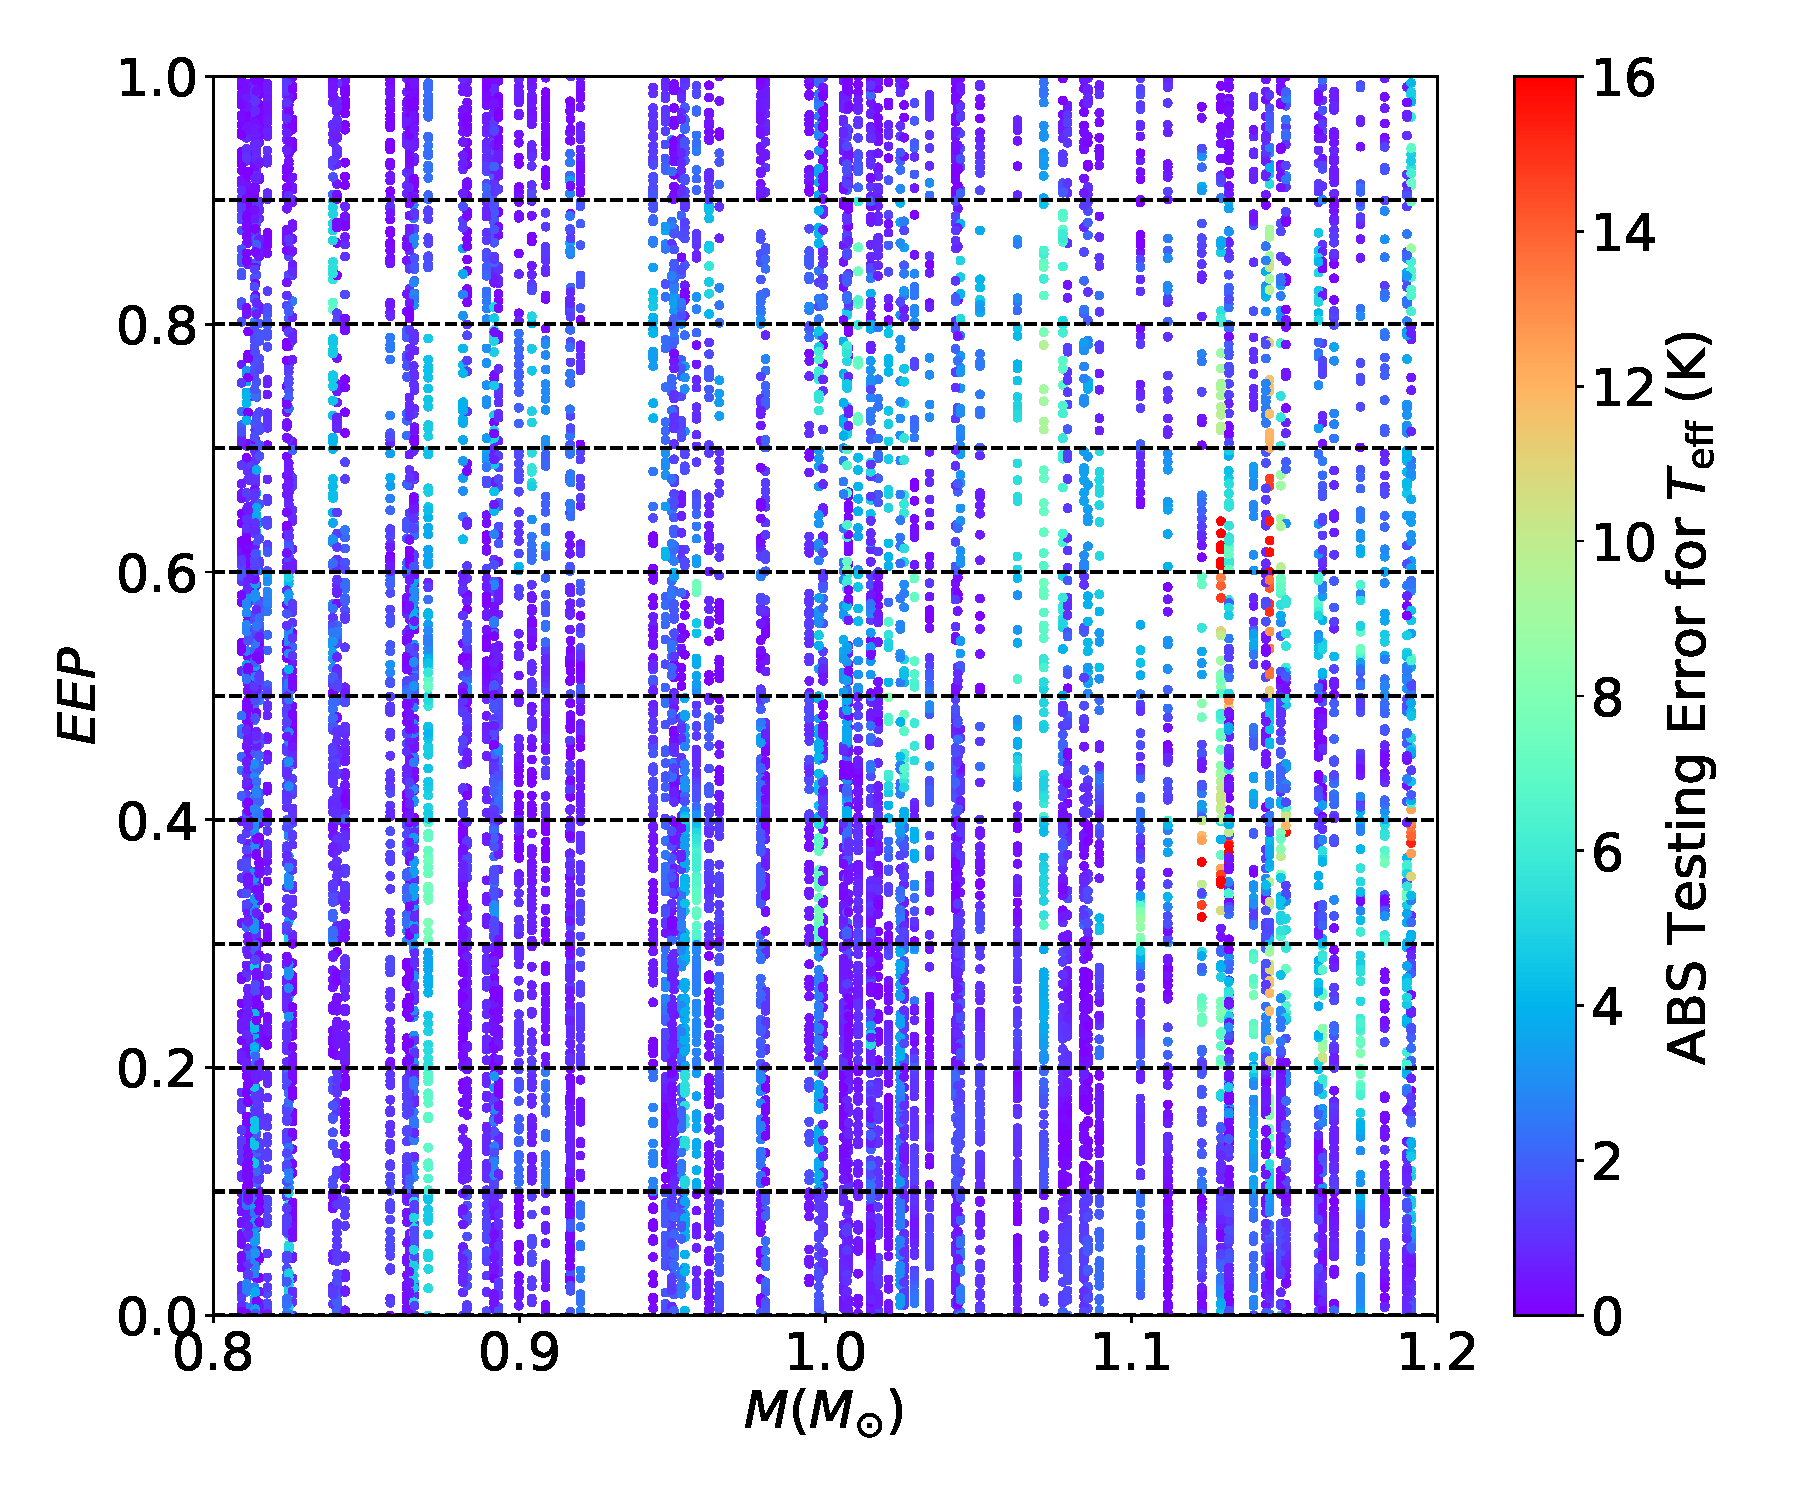
\includegraphics[width=1.0\columnwidth]{3d-testing_teff-10sections.pdf}
	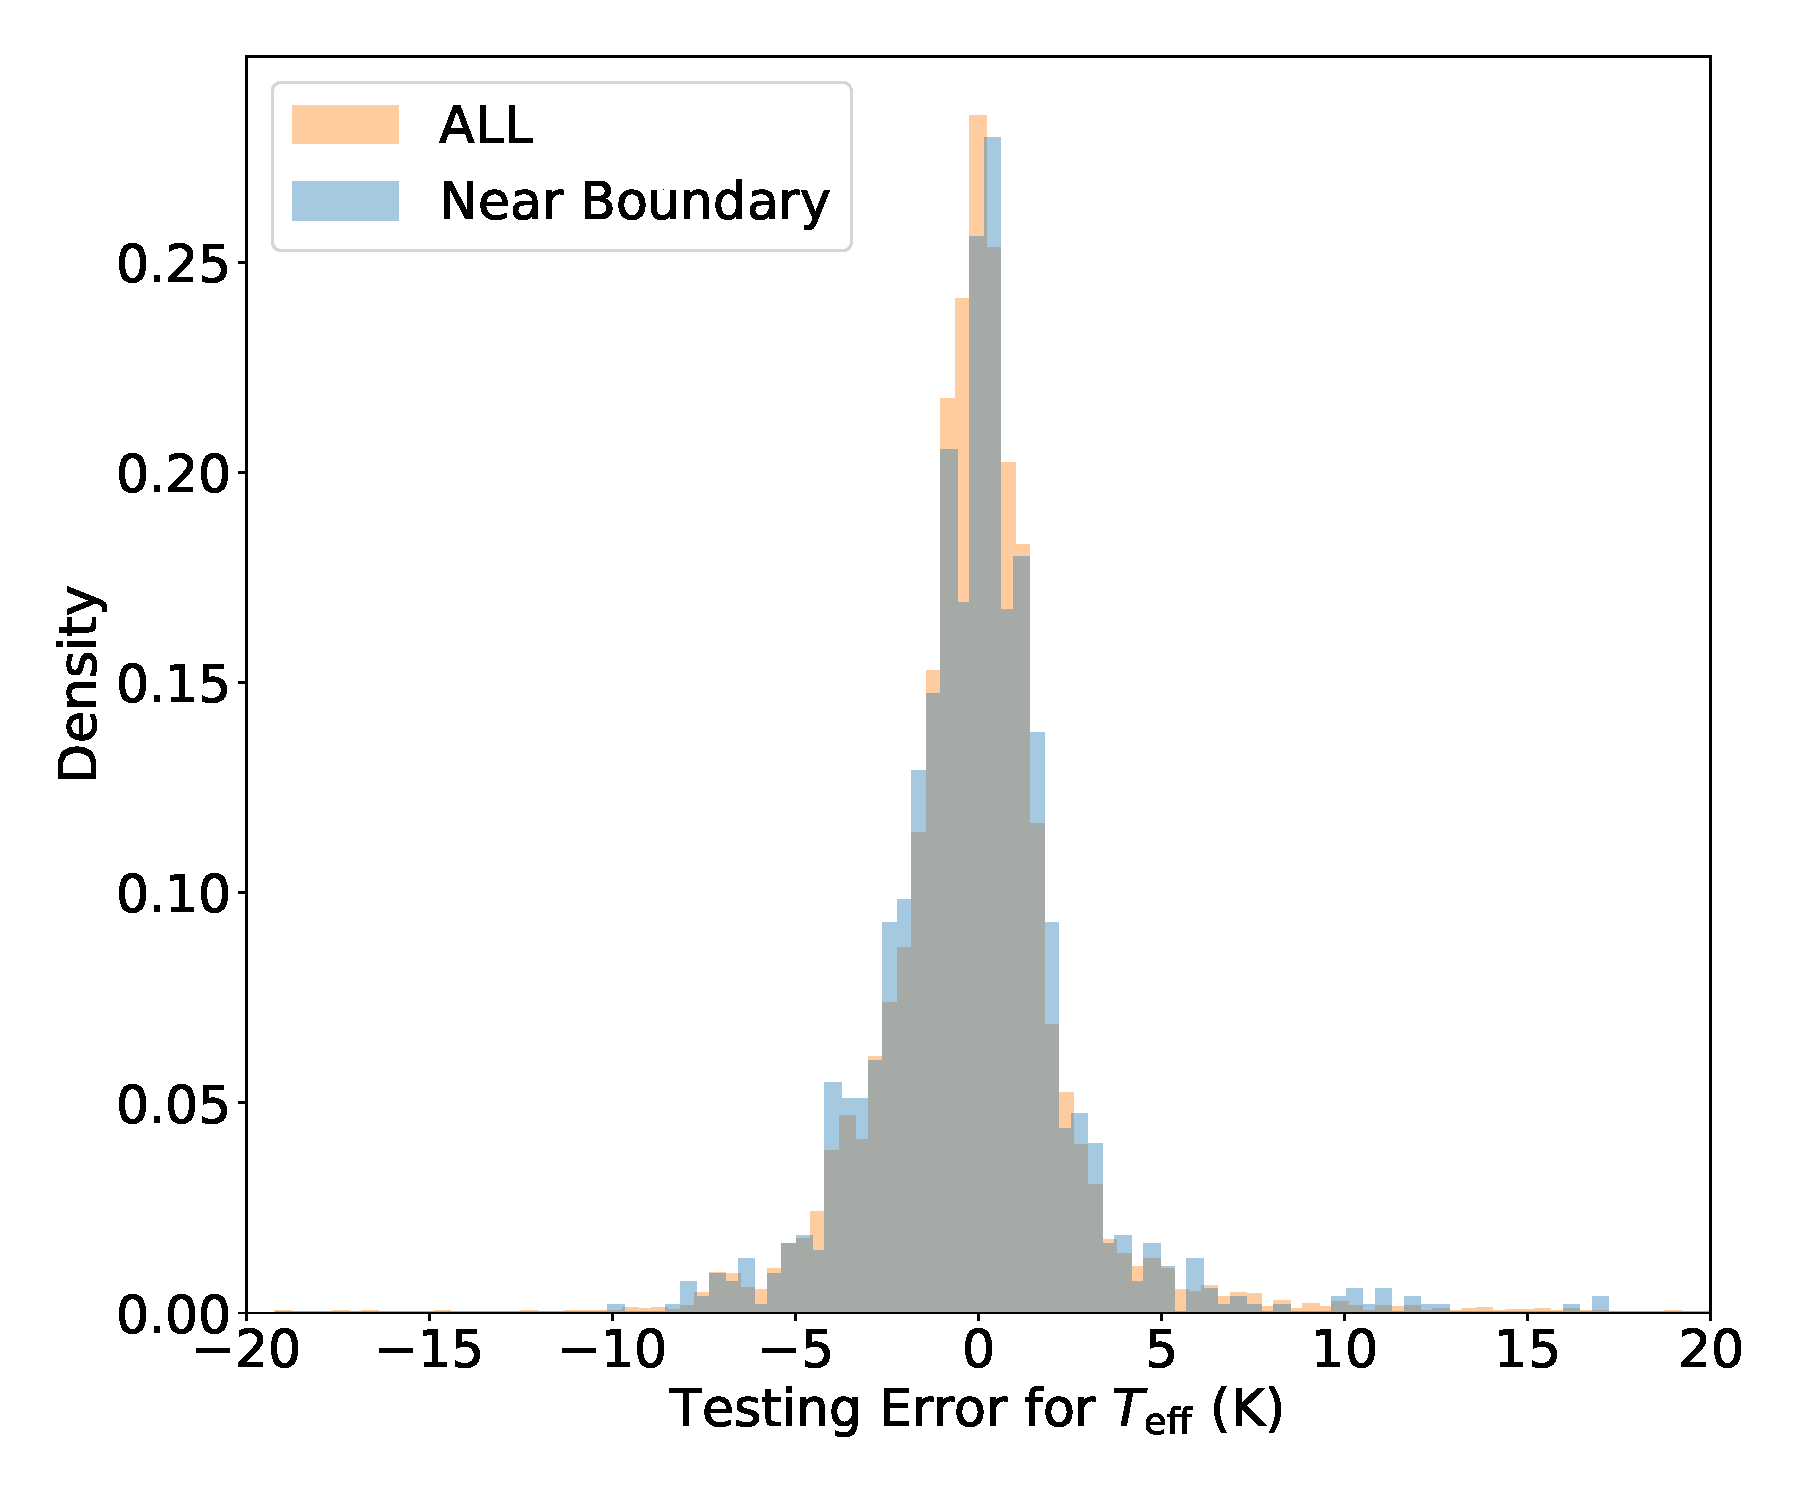
\includegraphics[width=1.0\columnwidth]{3d-testing_teff-hist-10sections.pdf}	
    \caption{Top: Testing errors of 3D GP model for $T_{\rm eff}$ on the $M - EEP$ diagram. Dashes indicates section boundaries. Bottom: examination of the edge effects of the section scenario. Probability distributions of testing errors of all testing data and those near the boundary ($\pm$0.01 EEP) in the upper graph are compared.  As it can be seen, testing errors do not raise around the boundary. }  
    \label{fig:3dtest}
\end{figure}


As mentioned above, the GPU memory captivity limits the actual number of data that induce the kernel function.   
This limit become critical for high-demission cases, because the parameter space exponentially increases with model demission and hence GP model accuracy inevitable declines. Improving GP models requires an increase of data points to induce kernels. 
%
A simple way is breaking the grid into sections and train GP models for each section separately. 
%The downside of this section scenario is that there will not be one GP model that maps the whole grid. However, as long as the goal of this work is augmenting a model grid but not deriving a universal function for stellar evolutions, this scenario is suitable. 
Here we test how this section scenario works for 3D GP models. We divide the dataset into 10 equal segments by $EEP$. We train one Exact GP model with 20,000 training data for each section. We then use the same testing dataset to quantify GP predictions for the five outputs, and the error index are averagely improved by around 10\%. For instance, the error index of $T_{\rm eff}$ decreases from 23.5 to 21.6 (1.7/5.0/14.9 K at 68/95/99.7\%). 
%

As expected, the section scenario improves GP models, but there is a major concern about the edge effects at the boundary between sections. If the GP model works significantly poorly at the section boundaries, it will be difficult to map the systematic errors across the whole parameter space. We examine this as illustrated in Figure~\ref{fig:3dtest}. We inspect absolute testing errors on the $M-EEP$ diagram (the top graph) and do not find obvious edge effects. We also do a statistical comparison between all testing errors and those around section boundaries ($\pm0.01EEP$) as demonstrated in the bottom graph. The density distributions of the two datasets are very similar and we hence conclude that there is no edge effect. The section scenario is adopted in the following study.  

Here we summary our set up for the GP model as follow:
\begin{itemize}
\item Model Type: Exact GP with the section scenario applied
\item Kernel: Mat32 (for all outputs)
\item Mean Function: Neural Network with 6 linear layers x 128 nodes and element-wise function (Elu) 
\item Likelihood Function: Gaussian Likelihood Function
\item Loss Function: Exact marginal likelihood
\item Optimiser: Adam including AMSGRAD variant
\item Early Stoping: controlled by the validating error index
\end{itemize}







     





